\renewcommand*{\arraystretch}{1.1}

\noindent\begin{tabularx}{17cm}{|>{\small \sf}c|X|}
	\hline
	query    & Interactive / complex / 8 \\ \hline
%
	title       & Recent replies \\ \hline
%
    pattern     & \hfill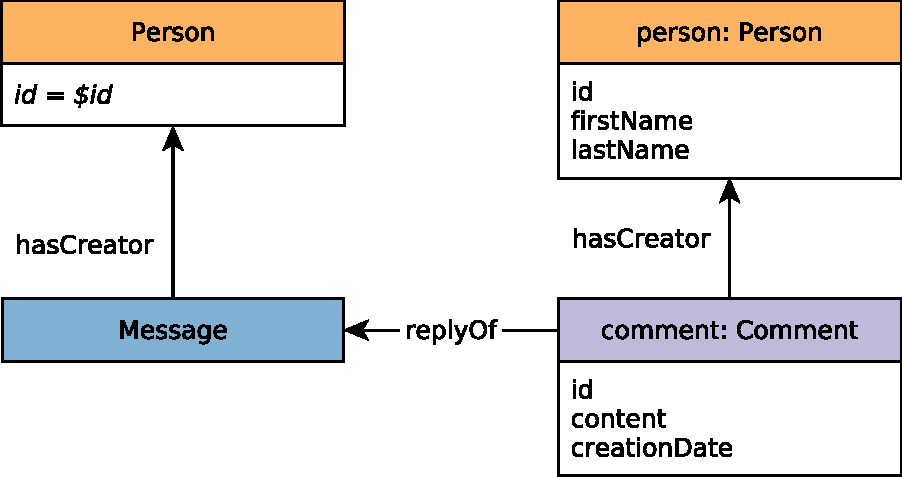
\includegraphics[scale=\patternscale,margin=0cm .2cm]{patterns/interactive-complex-read-08}\hfill\vadjust{} \\ \hline
%
	desc. & Given a start Person, find (most recent) Comments that are replies to
Messages of the start Person. Only consider immediate (1-hop) replies,
not the transitive (multi-hop) case. Return the reply Comments, and the
Person that created each reply Comment.
 \\ \hline
%
	
%
	params  &
	\vspace{1.1ex}{\begin{tabularx}{14.66cm}{|c|M|m{2cm}|Y|} \hline
	\cellcolor{parameter} \color{white} \footnotesize $\mathsf{1}$ & \varname{Person.id} & \cellcolor{gray!20} \vartype{ID} &  \\ \hline
	\end{tabularx}}\vspace{1.1ex} \\ \hline
%
	
	result      &
	\vspace{1.1ex}{\begin{tabularx}{14.66cm}{|c|M|m{2cm}|c|Y|} \hline
	\cellcolor{result} \color{white} \footnotesize $\mathsf{1}$ & \varname{Person.id} & \cellcolor{gray!20} \vartype{ID} &
	    \texttt{R} &
	     \\ \hline
	\cellcolor{result} \color{white} \footnotesize $\mathsf{2}$ & \varname{Person.firstName} & \cellcolor{gray!20} \vartype{String} &
	    \texttt{R} &
	     \\ \hline
	\cellcolor{result} \color{white} \footnotesize $\mathsf{3}$ & \varname{Person.lastName} & \cellcolor{gray!20} \vartype{String} &
	    \texttt{R} &
	     \\ \hline
	\cellcolor{result} \color{white} \footnotesize $\mathsf{4}$ & \varname{Comment.creationDate} & \cellcolor{gray!20} \vartype{DateTime} &
	    \texttt{R} &
	     \\ \hline
	\cellcolor{result} \color{white} \footnotesize $\mathsf{5}$ & \varname{Comment.id} & \cellcolor{gray!20} \vartype{ID} &
	    \texttt{R} &
	     \\ \hline
	\cellcolor{result} \color{white} \footnotesize $\mathsf{6}$ & \varname{Comment.content} & \cellcolor{gray!20} \vartype{String} &
	    \texttt{R} &
	     \\ \hline
	\end{tabularx}}\vspace{1.1ex} \\ \hline
	
%
	sort        &
	\vspace{1.1ex}{\begin{tabular}{|c|l|c|} \hline
	\cellcolor{sort} \color{white} \footnotesize $\mathsf{1}$ & \varname{Comment.creationDate} & \cellcolor{gray!20} $\desc$ \\ \hline
	\cellcolor{sort} \color{white} \footnotesize $\mathsf{2}$ & \varname{Comment.id} & \cellcolor{gray!20} $\asc$ \\ \hline
	\end{tabular}}\vspace{1.1ex} \\ \hline
	%
	limit       & 20 \\ \hline
	%
	CPs &
	\multicolumn{1}{>{\raggedright}l|}{
	  \chokepoint{2.4}, 
	  \chokepoint{3.2}, 
	  \chokepoint{3.3}, 
	  \chokepoint{5.3}
	  } \\ \hline
	%
    relevance &
      \small This query looks for paths of length two, starting from a given Person, going through its created Messages and
finishing at their replies. In this query there is temporal locality between the replies being accessed. Thus the top k
order by this can interact with the selection, i.e. do not consider older posts than the 20th oldest seen so far.
 \\ \hline%
\end{tabularx}
\vspace{2ex}